\documentclass[onecolumn,12pt]{article}
\usepackage[a4paper, total={7in, 9in}]{geometry}
\usepackage[utf8]{inputenc}
\usepackage[T1]{fontenc}
\usepackage{polski}
\usepackage{graphicx}
\usepackage{xcolor}
\usepackage{listings}



\usepackage{hyperref}
\hypersetup{
    colorlinks=false, %set true if you want colored link
    linktoc=all,     %set to all if you want both sections and subsections linked
}
\urlstyle{same}

\lstdefinestyle{yaml}{
     basicstyle=\color{blue}\footnotesize,
     rulecolor=\color{black},
     string=[s]{'}{'},
     stringstyle=\color{blue},
     comment=[l]{:},
     commentstyle=\color{black},
     morecomment=[l]{-}
 }

% Define Terraform language
\lstdefinestyle{terraform}{
  keywords={resource, variable, provider, output, module, locals, terraform, backend},
  sensitive=true,
  comment=[l]{\#},
  morecomment=[s]{/*}{*/},
  morestring=[b]",
  morestring=[b]',
  keywordstyle=\color{blue}\bfseries,
  commentstyle=\color{gray}\itshape,
  stringstyle=\color{red}
}

\begin{document}

% ----------Strona tytułowa------------
\begin{titlepage}
\begin{center}
\vspace*{2.5cm}
\Huge
\textbf{Spiderpool}
            
\vspace{0.5cm}
\LARGE
RDMA network solution for the Kubernetes
            
\vspace{1.5cm}

\large
Piotr Czarnik, Bartosz Kucharz
\\Gabriela Piwar, Wojciech Szmelich
              
\vspace{0.8cm}          
\Large
AGH Wydział Informatyki\\
2024    
\end{center}
\end{titlepage}

% ----------Spis treści------------
\tableofcontents
\thispagestyle{empty}
\newpage

% ----------Raport------------
\section{Wprowadzenie}
Kubernetes to jedno z najpopularniejszych narzędzi do zarządzania aplikacjami kontenerowymi. 
Z tego też względu nieustanie wprowadzane są nowe moduły usprawniające jego działanie. 

Jednym z nich jest Spiderpool - zaawansowane rozwiązanie zarządzania adresami IP (IPAM - IP Address Management) wykorzystujące technologię RDMA (Remote Direct Memory Access).
Rozszerza on standardowe interfejsy sieciowe kontenerów (CNI - Container Network Interface) umożliwiając tworzenie interfejsów Macvlan, Ipvlan, oraz SR-IOV.
Dzięki temu pozwala na większą dowolność w przypisywaniu adresów IP do kontenerów i w wykorzystaniu interfejsów sieciowych.
Natomiast SR-IOV umożliwia kontenerowi na bezpośredni dostęp do fizycznego interfejsu sieciowego - szybszy transfer danych między węzłami w klastrze Kubernetesa, minimalizacja opóźnienia i obciążenia procesora. 
Jest to szczególnie korzystne dla aplikacji wymagających wysokiej przepustowości i niskiego opóźnienia, 
jak aplikacje do przetwarzania dużych ilości danych, middleware, CNF (Container Network Functions) czy systemy baz danych.

\section{Opis technologii}

\subsection{Kubernetes}
Spiderpool działa na klastrach, czyli zestawie maszyn (węzłów) do uruchamiania skonteneryzowanych aplikacji. Kubernetes jest platformą open source do zarządzania takimi klastrami. Służy do zarządzania zadaniami i serwisami uruchamianymi w kontenerach, oraz umożliwia deklaratywną konfigurację i automatyzację. Najmniejsza i najprostsza jednostka w środowisku Kubernetes to pod, czyli grupa jednego lub wielu kontenerów aplikacji. 
W ''czystym'' k8s kontenery wewnątrz poda współdzielą adres IP i przestrzeń portów, zawsze są uruchamiane wspólnie w tej samej lokalizacji i współdzielą kontekst wykonawczy na tym samym węźle.

\subsection{AWS}
Spiderpool jest stworzone z myślą o działaniu na dowolnym środowisku chmurowym. Ułatwia również zarządzanie takimi rozwiązaniami jak multicloud czy chmura hybrydowa.\\
Jedną z najbardzej znanych i używanych platform chmurowych jest Amazon Web Services (AWS), która zapewnia szeroki wybór usług oraz zasobów obliczeniowych, sieciowych i przechowywania danych. Usługi Amazona są znacznie  rozbudowane i umożliwiają skonfigurowanie środowiska w taki sposób, aby było jak najbardziej dopasowane do danych potrzeb. Jedną z najważniejszych usług dostępnych w AWS jest Elastic Compute Cloud (EC2), która umożliwia elastyczne skalowanie zasobów obliczeniowych. Szerokie zastosowanie tej platformy oznacza również, że istnieje ogromna ilość informacji, dokumentacji i pomocy dostępnych dla użytkowników. Dlatego zdecydowano się wdrożyć projekt na tym środowisku.

\subsection{Ansible}
Ansible jest silnikiem orkiestracji pozwalającym na tworzenie oprogramowania w paradygmacie ,,infrastructure as a code''.
Umożliwia automatyzację provisioningu, konfiguracji i deploymentu systemów oraz oprogramowania za pomocą Playbook-ów - zestawów tasków, które mają się wykonać na wcześniej zdefiniowanych node'ach.

Ansible udostępnia moduły dedykowane do konfiguracji AWSa i Kubernetesa.
Wartą uwagi cechą playbooków jest idempotentność operacji - taski sprawdzają, czy dane zadanie już nie zostało wykonane, a jeśli tak to go nie powtarzają - umożliwia to wielokrotne ich uruchamianie bez konieczności czyszczenia całego środowiska.

\section{Case Study - opis projektu}
Za pomocą wymienionych uprzednio technologii, dążymy do uzyskania automatycznego deploymentu środowiska Spiderpool na chmurze AWS za pomocą Ansible'a.
W miejscach, gdzie użycie natywnych Ansible'owych modułów nie będzie możliwe, wykorzystane zostaną skrypty bash-owe lub (co jest bardziej preferowane) skrypt bash-owy wewnątrz playbooka.

Po deploymencie Spiderpoola konieczne jest zautomatyzowanie sprawdzenia poprawności działania środowiska:
\begin{enumerate}
    \item test łączności sieciowej między kontenerami - za pomocą ping-ów lub curl-ów,
    \item test działania funkcjonalności Spiderpoola - dodawanie i uwalnianie adresów IP,
    \item uruchomienie kilku przykładowych aplikacji web-wych w kontenerach używających różnych adresów IP za pomocą Macvlan lub Ipvlan.
\end{enumerate}

W ramach projektu zautomatyzowane zostaną więc:
\begin{enumerate}
    \item konfiguracja AWS - VPC i EC2,
    \item deployment K8s,
    \item deployment Spiderpoola,
    \item testy, a w tym deployment przykładowych aplikacji.
\end{enumerate}

\section{Architektura rozwiązania}
Spiderpool składa się z następujących komponentów:
\begin{enumerate}
    \item Kontroler Spiderpoola, odpowiedzialny za interakcje z API Server. 
    Zarządza różnymi zasobami CRD; SpiderIPPool, SpiderSubnet, SpiderMultusConfig; poprzez ich walidację, tworzenie i update-owanie ich statusu. 
    Dodatkowo odpowiada na żądania od Spiderpool-agent Pods, takie jak alokacja, zwolnienie czy zarządzanie pulą adresów IP. 
    \item Spiderpool-agent, zestaw daemon-ów działających na każdym nodzie. 
    Wspiera instalacje wtyczek takich jak Multus, Coordinator, IPAM, czy CNI. 
    Odpowiada na żądania alokacji IP przez CNI, podczas tworzenia Pod-u. 
    Komunikuje się z Spiderpool-controller w zakresie alokacji i tworzenia IP Pod-u. 
    Komunikuje się także z Coordinator w zakresie synchronizacji konfiguracji i wspierania implementacji alokacji IP.
    \item Wtyczek CNI
    \newline Spiderpool IPAM plugin, główny CNI używany do zarządzania alokacją adresów IP.
    \newline Coordinator plugin, odpowiada za koordynację routingu, połączenie pomiędzy hostami. 
    Zapewnia unikalność adresów IP, odpowiednią adresacje MAC.
    \newline Ifacer plugin, automatyzuje tworzenie wirtualnych interfejsów dla VLAN-ów i Bondów (łączenia wielu interfejsów sieciowych w jedno logiczne połączenie).
    \newline Multus CNI, zarządza (scheduler) innymi wtyczkami CNI.
    \item Komponentów SR-IOV
    \item Komponentów RDMA
    \newline RDMA CNI, implementuje izolację sieci
\end{enumerate}


\section{Konfiguracja środowiska}

W celu realizacji założeń projektowych związanych z automatycznym deploymentem Spiderpoola 
przeprowadzono konfigurację środowiska w AWS. Umożliwił to dostęp do platformy AWS Academy Learner
Lab gdzie w ramach projektu otrzymaliśmy 100 dolarów w zasobach do wykorzystania na platformie. 

Koniecznym krokiem było podłączenie konta w AWS do środowiska na maszynie lokalnej. Wystarczy skopiować
plik \textit{credentials}, dostępny w  sekcji AWS Details w Learner Lab do folderu textit{~/.aws/
credentials}.

\begin{figure}
    \centering
    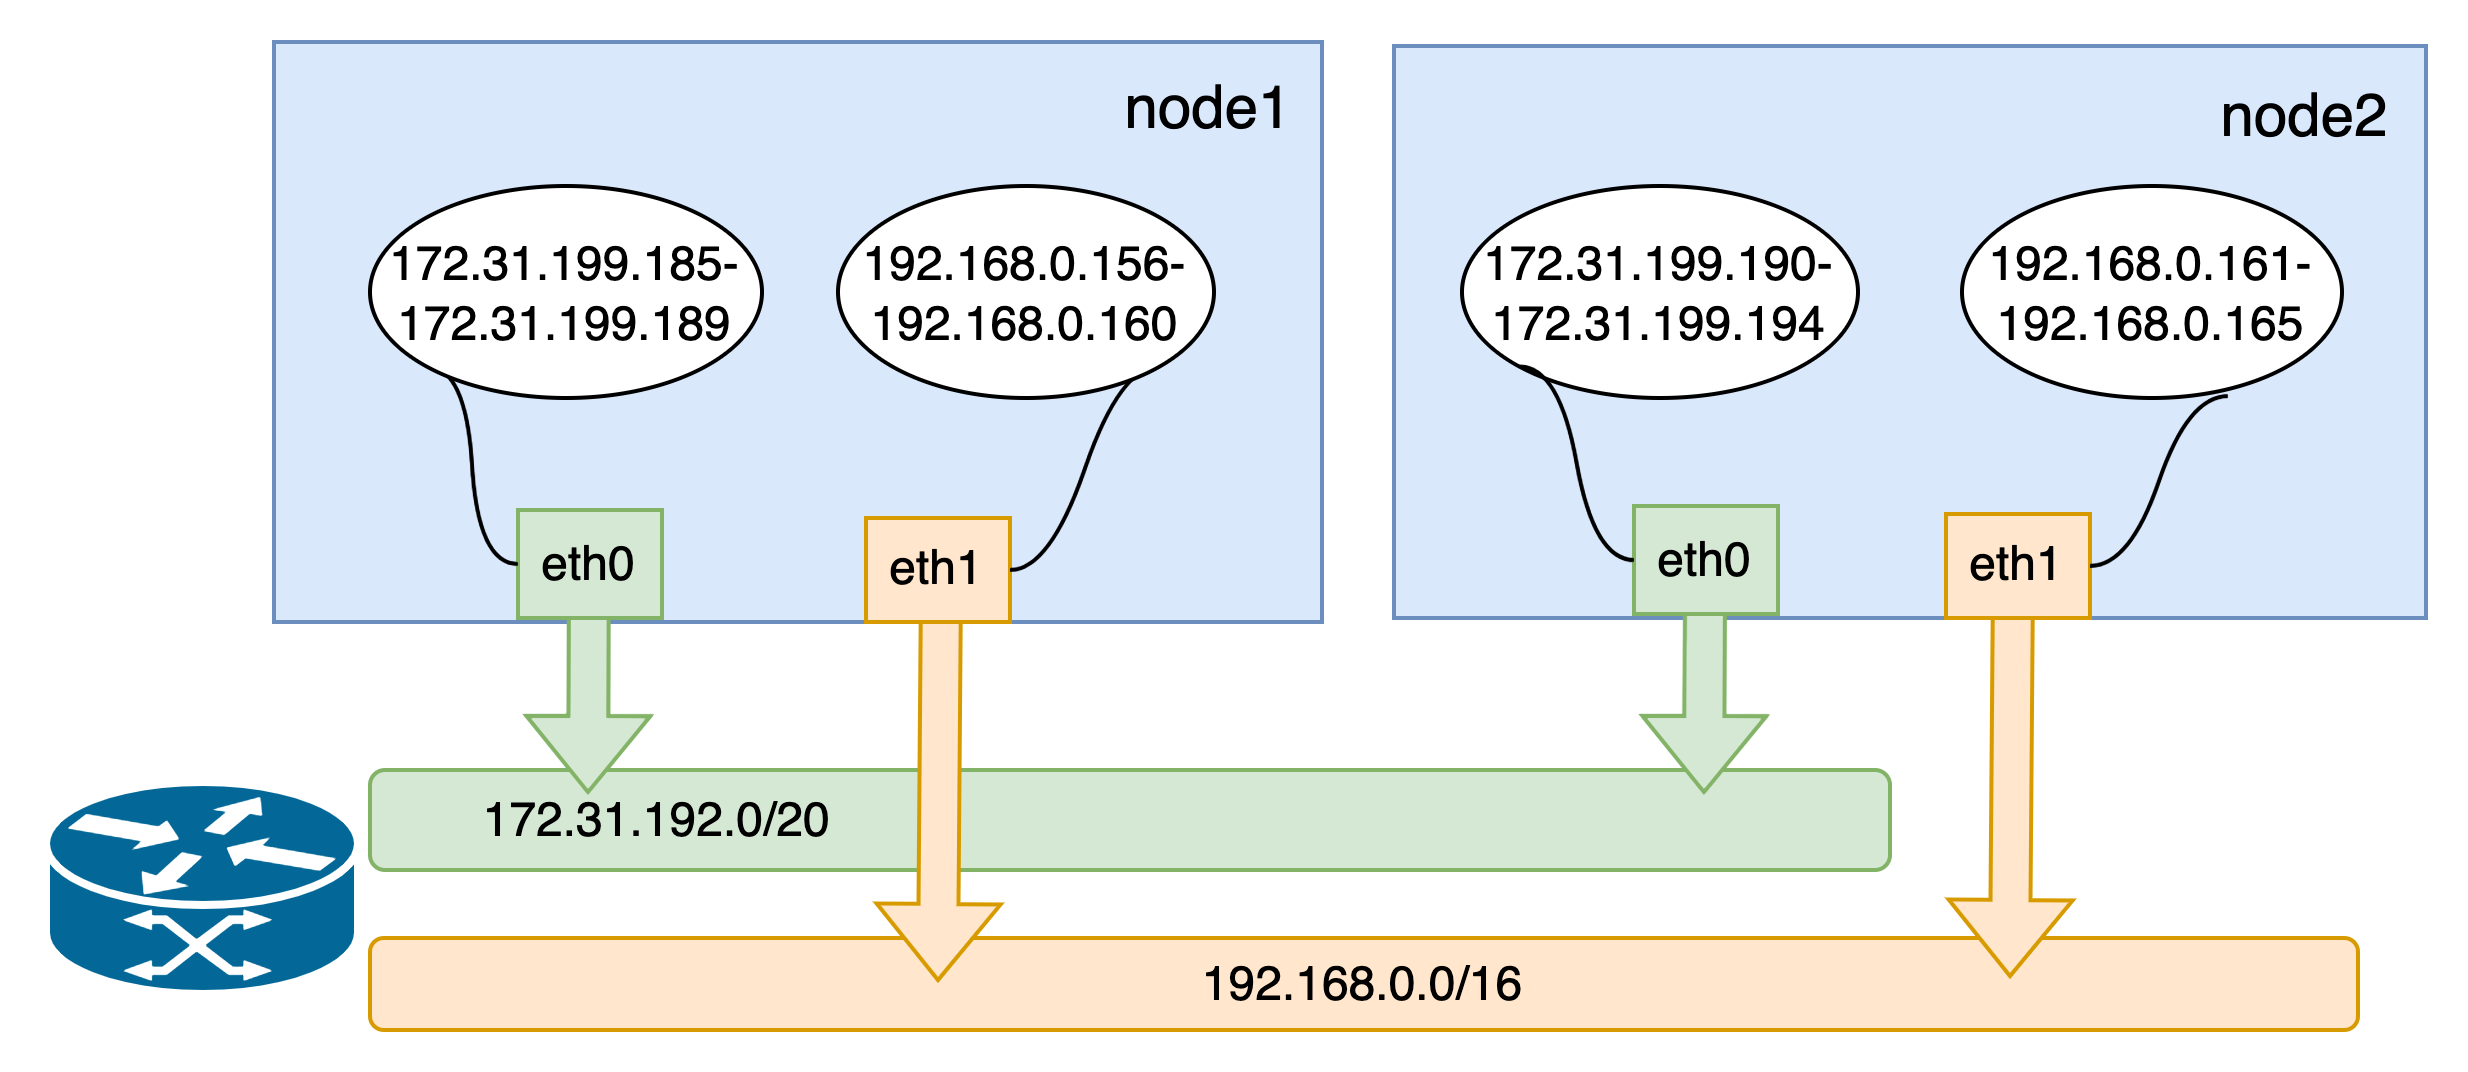
\includegraphics[width=0.8\linewidth]{alicloud-k8s-network_NOT_OURS.png}
    \caption{Schemat przedstawiający uzyskaną konfigurację.}
    \label{fig:enter-label}
\end{figure}

\section{Instalacja}

Aby zainstalować nasz projekt, na początek należy spełnić kilka wymagań. Przede wszystkim 
potrzebne jest konto AWS z odpowiednimi uprawnieniami. Konieczne jest również zainstalowanie
Terraform w wersji 0.12 lub nowszej oraz Ansible w wersji 2.9 lub nowszej. Dodatkowo, wymagane
jest posiadanie pary kluczy SSH umożliwiających dostęp do instancji EC2 na platformie AWS.

Proces instalacji rozpoczyna się od klonowania repozytorium projektu z zdalnego repozytorium 
oraz przejścia do katalogu z projektem. W tym celu należy użyć poleceń:

\begin{verbatim}
git clone https://github.com/gpiwar/suu_spiderpool_project.git
cd suu_spiderpool_project
\end{verbatim}

Głównym krokiem instalacji jest uruchomienie skryptu \textit{run.sh}, który w pełni automatycznie przeprowadza proces konfiguracji infrastruktury oraz wdrażania aplikacji. Skrypt ten tworzy środowisko, wdrażając klaster Kubernetes oraz aplikacje takie jak Spiderpool i Multus CNI. Również wykonuje niezbędne komendy Terraform i Ansible. Ponadto przeprowadza on cały proces instalacji, w tym konfigurację sieci, instancji EC2 oraz wdrożenie aplikacji w klastrze Kubernetes.

\section{Proces tworzenia aplikacji}
Opisać kod - w zależności co ważne dodać fragmenty, narazie wstawiłam puste miejsca na kod

\subsection{Terraform}

\subsubsection{Adresy sieci}
\begin{lstlisting}[style=terraform]
variable "net_cidr" {
  type        = string
  description = "Network CIDR"
  default     = "172.31.0.0/16"
}

variable "public_subnet_cidr" {
  type        = string
  description = "Public Subnet CIDR"
  default     = "172.31.0.0/20"
}

variable "private_subnet_cidrs" {
  type        = list(string)
  description = "Private Subnet CIDRs"
  default     = ["172.31.16.0/20", "172.31.64.0/20", "172.31.96.0/20"]
}

locals {
  bastion = {
    ami           = data.aws_ami.this.id
    instance_type = "t2.micro"
  }
  interfaces = {
    master_eth0 = {
      subnet_id = aws_subnet.private[0].id
      ip_list   = ["172.31.17.1"]
    }
    worker1_eth0 = {
      subnet_id = aws_subnet.private[1].id
      ip_list   = [for i in range(1, 5) : "172.31.65.${i}"]
    }
    worker1_eth1 = {
      subnet_id = aws_subnet.private[2].id
      ip_list   = [for i in range(1, 5) : "172.31.97.${i}"]
    }
    worker2_eth0 = {
      subnet_id = aws_subnet.private[1].id
      ip_list   = [for i in range(1, 5) : "172.31.66.${i}"]
    }
    worker2_eth1 = {
      subnet_id = aws_subnet.private[2].id
      ip_list   = [for i in range(1, 5) : "172.31.98.${i}"]
    }
    worker3_eth0 = {
      subnet_id = aws_subnet.private[1].id
      ip_list   = [for i in range(1, 5) : "172.31.67.${i}"]
    }
    worker3_eth1 = {
      subnet_id = aws_subnet.private[2].id
      ip_list   = [for i in range(1, 5) : "172.31.99.${i}"]
    }
    worker4_eth0 = {
      subnet_id = aws_subnet.private[1].id
      ip_list   = [for i in range(1, 5) : "172.31.68.${i}"]
    }
    worker4_eth1 = {
      subnet_id = aws_subnet.private[2].id
      ip_list   = [for i in range(1, 5) : "172.31.100.${i}"]
    }
  }
}
\end{lstlisting}
Zmienne określają adresy dla sieci VPC, publicznych podsieci oraz grupę adresów dla sieci prywatnych. Następnie za pomocą wartości lokanych ustawiany jest adress bastionu oraz pule adresów IP dla interfejsów. Każdy z czterech workerów posiada dwa interfejsy eth0 i eth1.

\subsubsection{Pobieranie informacji obrazie}
\begin{lstlisting}[style=terraform]
data "aws_ami" "this" {
  most_recent = true
  filter {
    name   = "owner-alias"
    values = ["amazon"]
  }

  filter {
    name   = "name"
    values = ["RHEL-9.4*"]
  }
}
\end{lstlisting}


Pobranie danych o najnowszym obrazie AMI RHEL-9.4 od Amazona.

\subsubsection{Grupy bezpieczeństwa}
Główna grupa bezpieczeństwa konfiguruje regułę egress, pozwalającą na cały ruch do wszystkich adresów IP. Reguła igress, pozwala natomiast jedynie na komunikacje przez SSH.

W przypadku grupy wewnątrz klastra dopuszczony jest ruch dla wszystkich protokołów na wszystkich portach i adresach IP.



\subsubsection{cluster.tf}
Ten plik zawiera konfiguracje klastra. Wykorzystuje zmienne zdefiniowane w pliku variables.tf aby utworzyć zasoby określające m.in. łączenie się z klastrem, gateway NAT, podsieci, interfejsy sieciowe.

\subsection{Manifests}

\textbf{SpiderMultusConfig.yaml}
\begin{lstlisting}[style=yaml]
---
apiVersion: spiderpool.spidernet.io/v2beta1
kind: SpiderMultusConfig
metadata:
  name: ipvlan-eth0
  namespace: kube-system
spec:
  cniType: ipvlan
  ipvlan:
    master:
    - eth0
---
apiVersion: spiderpool.spidernet.io/v2beta1
kind: SpiderMultusConfig
metadata:
  name: ipvlan-eth1
  namespace: kube-system
spec:
  cniType: ipvlan
  ipvlan:
    master:
    - eth1
\end{lstlisting}

\textbf{SpiderIPPool.yaml}
\begin{lstlisting}[style=yaml]
\end{lstlisting}


\textbf{Deployment-nginx.yaml}
\begin{lstlisting}[style=yaml]
\end{lstlisting}


\textbf{Deployment-busybox.yaml}
\begin{lstlisting}[style=yaml]
\end{lstlisting}


\subsection{Ansible - playbooks}
%Za pomocą Ansible dokonujemy deployu \newline
\textbf{pre-deploy.yml} \newline
Dokonujemy konfiguracji połączenia z bastionem i klustrem. Dodajemy klucz ssh, ustawiamy hostname, dodajemy cluster IPs do /etc/hosts. Następnie instalujemy następujące aplikacje vim, tmux, git, bash-completion, python3-pip.
\begin{lstlisting}[style=yaml]
\end{lstlisting}


\textbf{deploy-k8s.yml} \newline
Dokonujemy instalacji kubernetesa, CRI-O, container-selinux, cri-o, kubelet, kubeadm, kubectl.
\begin{lstlisting}[style=yaml]
\end{lstlisting}

\textbf{deploy-spiderpool.yml} \newline
Dokonujemy instalacji helm-a. Za pomocą helm-a instalacji spiderpool-a. Następnie dodajemy pulę adresów IP do spiderpool-a. Playbook realizuje komendy
\begin{lstlisting}
helm repo add spiderpool https://spidernet-io.github.io/spiderpool

helm repo update spiderpool

helm install spiderpool spiderpool/spiderpool --namespace kube-system \
--set ipam.enableStatefulSet=false \
--set multus.multusCNI.defaultCniCRName="ipvlan-eth0"

\end{lstlisting}



\textbf{deploy-apps.yml} \newline
Dokonujemy deploymentu busybox, nginx.
\begin{lstlisting}[style=yaml]
    - name: Get Spiderpool IP pools
      ansible.builtin.command: kubectl get spiderippools.spiderpool.spidernet.io
      register: kubectl_get_spiderippools
      changed_when: false

    - name: Get busybox pod names
      ansible.builtin.command: kubectl get pods -oNAME --selector=run=busybox
      register: busybox_pod_names
      changed_when: false

    - name: Get IPs from inside of busybox pods
      ansible.builtin.command: "kubectl exec -it {{ item }} -- ip -4 addr show scope global"
      loop: "{{ busybox_pod_names.stdout_lines }}"
      register: busybox_pods_ips
      changed_when: false
\end{lstlisting}


\section{Demo aplikacji}
Aby przetestować w pełni poprawne działanie proponowanego rozwiązania konieczne jest uruchomienie
demo naszej aplikacji wykorzystującej Spiderpool. Poniżej przedstawiono odpowiednie kroki.

\subsection{Konfiguracja}

Aby przeporwadzić demo naszej aplikacji wykorzystującej Spiderpool, należy skonfigurować AWS, 
zamieszczając plik credentials.txt w odpowiednim katalogu. Jest to niezbędne to prawidłowego działania
przedstawionego rozwiązania. 

\subsection{Przygotowanie danych}

W trakcie testowania możliwa jest edycja pliku \textit{'variables.tf'}, w celu dodania nowego workera do klastra. Jeżeli zdecydujemy się na ten krok należy dodać również nowe interfejsy sieciowe w sekcji \textit{interfaces}, gdzie przypiszemy odpowiednie adresy IP do interfejsów 'etho0' i etho1'. Kolejnym 
i ostatnim krokiem jest aktualizacja pliku \textit{'SpiderIPPool.yaml'}, gdzie dodamy nowe adresy IP.
Poniżej przedstawiono przykładowe definicje workera i jego interfejsów:

\begin{lstlisting}[style=yaml]

    worker4 = {
      ami           = data.aws_ami.this.id
      instance_type = "t2.large"
      interfaces = [
        aws_network_interface.this["worker4_eth0"].id,
        aws_network_interface.this["worker4_eth1"].id
      ]
    }
--------------------------------

    worker4_eth0 = {
      subnet_id = aws_subnet.private[1].id
      ip_list   = [for i in range(1, 5) : "172.31.68.${i}"]
    }
    worker4_eth1 = {
      subnet_id = aws_subnet.private[2].id
      ip_list   = [for i in range(1, 5) : "172.31.100.${i}"]
    }
\end{lstlisting}

\subsection{Uruchomienie skryptu}

Tak jak opisano w sekcji z instalacją, do wdrożenia aplikacji konieczne jest pobranie plików z 
repozytorium projektowego na platformie GitHub. Po przejściu do pobranego folderu należy 
uruchomić skrypt \textit{run.sh}, który automatycznie zainstaluje i skonfiguruje konieczne pliki.

\subsection{Sprawdzenie działania}
Po zakończeniu procesu wdrażania, należy zweryfikować wyniki. W konsoli zarządzania AWS można
sprawdzić, czy zostały utworzone odpowiednie zasoby, takie jak VPC, podsieci, instancje EC2 oraz
inne elementy infrastruktury. Następnie, za pomocą narzędzia kubectl, można ręcznie sprawdzić stan
klastra Kubernetes, w tym węzłów i podów, używając poleceń przedstawionych poniżej.

\begin{verbatim}
kubectl get nodes
kubectl get pods
kubectl exec -it {{ item }} -- ip -4 addr show scope global
\end{verbatim}

Gdzie w miejsce 'item' wpisujemy konkretne pody otrzymane po wywołaniu poprzenich poleceń.
Na końcu sprawdzamy czy Spiderpool poprawnie przypisał adresy IP z zdefiniowanych pul do podów. 

\section{Podsumowanie}

Podsumowując, skrypt stworzony na potrzeby projektu dostarcza skutecznych narzędzi do zarządzania siecią kontenerową w środowiskach Kubernetes. Realizowany projekt jest automatycznym rozwiązaniem
dla możliwości narzędzia Spiderpool. Dzięki integracji z technologiami, takimi jak AWS, Ansible, oraz Terraform, rozwiązanie zapewnia elastyczność, skalowalność i efektywność. W ramach projektu przetestowano funkcjonalność Spiderpoola, sprawdzając poprawność alokacji adresów IP oraz 
działanie aplikacji webowych wdrożonych w kontenerach z różnymi konfiguracjami sieciowymi.

%\bibliography{}

\end{document}